\documentclass[lecture_notes.tex]{subfiles}

\begin{document}

\notestitle{Session 1}{Classical Magnetism and Mean-Field Theory}%
  {classical\_magnetism.ipynb}{none (second quantization is introduced from scratch)}

\section*{Contents and goals}
In this session we build the minimal machinery we need to talk about interacting electrons,
second quantization, and we use it to answer a very concrete question: when do repulsive
electron--electron interactions spontaneously break a symmetry of the Hamiltonian? We will look
at two symmetry-broken phases, classical magnetism and charge density waves, and we will treat
both of them entirely at the mean-field level. By the end of the session we will see a case
where mean-field theory demonstrably gives us the wrong ground state, the Hubbard dimer, and
that failure is precisely what motivates the exact-diagonalization and tensor-network methods
we develop in the rest of the course.

\section*{Learning outcomes}
By the end of this session, you should be able to:
\begin{itemize}[nosep]
  \item Write single-particle and many-body Hamiltonians in second-quantized form, and explain
    why the interaction term makes the many-body problem exponentially hard.
  \item Set up and run a mean-field self-consistency loop for the Hubbard and CDW models, and
    interpret the resulting exchange splitting, gap, and order parameter.
  \item Derive the superexchange coupling $J\sim t^2/U$ from degenerate perturbation theory and
    use it to predict collinear versus frustrated classical spin order.
  \item Identify when mean-field theory fails qualitatively, and explain why, using the
    entangled singlet ground state of the Hubbard dimer as the counterexample.
\end{itemize}

\section{Single-particle versus many-body Hamiltonians}
Let us start by distinguishing two broad classes of electronic Hamiltonians. The first class is
what we call single-particle Hamiltonians: they are bilinear in the field operators,
\begin{equation}
  \Ham_0 = \sum_{ij} t_{ij}\, \cre{i}\ann{j},
\end{equation}
where $t_{ij}$ is a hopping amplitude that we can think of as the probability amplitude for an
electron in orbital $j$ to jump to orbital $i$. Because $\Ham_0$ is just a matrix acting on a
single-particle Hilbert space, every electron here moves essentially independently of the
others, and finding the spectrum is nothing more than diagonalizing an $L\times L$ matrix for
$L$ orbitals. This is already enough to describe a wide variety of materials: insulators,
semiconductors, ordinary metals.

The case we actually care about most, though, is the many-body case. Here we again have the
bilinear term, but we also add a term that is quartic in the fermionic operators,
\begin{equation}
  \Ham = \Ham_0 + \sum_{ijkl} V_{ijkl}\, \cre{i}\cre{j}\ann{k}\ann{l},
  \label{eq:generalH}
\end{equation}
and $V_{ijkl}$ tells us the strength of this interaction. This is the term that is responsible
for essentially all of the exotic phenomena we care about in quantum materials: magnetism,
charge density waves, superconductivity, and every strongly correlated phase we will meet later
in the course. What makes second quantization so useful is that it lets us write both the
single-particle and the many-body piece of Eq.~\eqref{eq:generalH} in one common language.

\section{Second quantization}
So let us set up that language. We define the fermionic annihilation and creation operators
$\ann{i}$, $\cre{i}$ for orbital $i$, and a vacuum state $\vac$ that has no electrons at all,
$\ann{i}\vac = 0$ for every $i$. You can think of the vacuum as a vector and of the operators as
matrices that map one vector to another; a single-particle basis state is simply $\cre{i}\vac$,
and the matrix elements of $\Ham_0$ in this basis are exactly the hopping amplitudes $t_{ij}$ we
started with.

How do we enforce, mathematically, that no site can hold more than one electron of a given
species? We impose the canonical anticommutation relations,
\begin{equation}
  \{\ann{i},\cre{j}\} = \delta_{ij}, \qquad \{\ann{i},\ann{j}\} = \{\cre{i},\cre{j}\} = 0.
  \label{eq:anticomm}
\end{equation}
This single algebraic statement does two things at once: swapping two fermions picks up a minus
sign, which is exactly antisymmetry of the wavefunction, and acting with $\cre{i}$ twice on any
state gives zero, which is exactly the Pauli exclusion principle. Throughout the course we will
meet three flavors of local degree of freedom built this way:
\begin{itemize}[nosep]
  \item \textbf{Spinful fermions}: each site has four possible states, $\ket{0}$, $\ket{\up}$,
    $\ket{\dn}$, $\ket{\up\dn}$. This is the realistic case, the one you would use for something
    like a hydrogen atom.
  \item \textbf{Spinless fermions}: each site has only two states, $\ket{0}$ and $\ket{1}$.
    Formally, a spinful fermion is really nothing more than two decoupled spinless fermions, one
    per spin flavor.
  \item \textbf{Spin-$\tfrac12$ operators}: again two states, $\ket{\up}$ and $\ket{\dn}$, but
    now the operators are \emph{bosonic}: they commute on different sites instead of
    anticommuting. As we will see in Section~\ref{sec:strongcoupling}, a local spin emerges
    naturally from a spinful fermion once we project out double occupancy and the empty state.
    This is the origin of what is called spin--charge separation.
\end{itemize}

\begin{notebook}
Open \texttt{classical\_magnetism.ipynb}, section ``Bandstructure of a tight binding chain'' and
``Finite size chains.'' Diagonalize $\Ham_0$ for a chain of $L$ sites and check for yourself
that the number of eigenvalues grows linearly in $L$, while their spacing shrinks: this is the
discrete precursor of a continuous band. Then, in ``Density of states of a finite system as a
function of the system size,'' plot the density of states, $\rho(\omega) =
-\tfrac1\pi\,\Im\Tr\,[\omega - \Ham_0 + i0^+]^{-1}$, and think about how it connects to what a
tunneling-spectroscopy or ARPES experiment actually measures.
\end{notebook}

\section{Worked example: the tight-binding dimer}
\label{sec:dimer}
Before we add any interactions, it is worth solving the smallest possible chain by hand, since
we will keep coming back to it. Take $L=2$ sites with hopping $t$, and let us include spin from
the start, so each site can hold a spin-up and a spin-down electron independently:
\begin{equation}
  \Ham_0 = -t \sum_\sigma \left(\cre{0\sigma}\ann{1\sigma} + \cre{1\sigma}\ann{0\sigma}\right).
\end{equation}
Spin never enters the hopping, so $\Ham_0$ splits into two identical $2\times2$ spinless
problems, one per spin flavor:
\begin{equation}
  \Ham_0^{(\sigma)} = -t\begin{pmatrix} 0 & 1 \\ 1 & 0\end{pmatrix}
  \;\Longrightarrow\;
  \varepsilon_{\pm} = \mp t, \qquad
  \ket{\pm} = \frac{1}{\sqrt2}\left(\ket{0} \pm \ket{1}\right).
\end{equation}
We call $\ket{+}$ the \textbf{bonding} orbital, at energy $-t$, and $\ket{-}$ the
\textbf{antibonding} orbital, at energy $+t$. Now restore spin: each of these two orbital levels
can separately hold a spin-up and a spin-down electron, so we actually have $2\times 2 = 4$
single-particle eigenstates in total, even though there are only \emph{two} distinct energies,
$\pm t$, each doubly degenerate. This is the direct answer to a question you may have already
asked yourself while looking at the notebook: why four eigenstates for two sites, and why are
some of them degenerate? The degeneracy is counting spin, not orbital content, and it follows
from the fact that $\Ham_0$ commutes with total spin: nothing in $\Ham_0$ distinguishes $\up$
from $\dn$.

If we fill in electrons one at a time starting from $\ket{\Omega}$, we generate the full
many-body basis for two spinful sites, exactly as we set up in the previous section. At half
filling with two electrons, for instance, there are $\binom{4}{2}=6$ states in total: four of
them are singly occupied ($\up\dn$, $\dn\up$, $\up\up$, $\dn\dn$, one electron per site) and two
of them are doubly occupied (both electrons on the same site). Keep this counting in mind, since
it is exactly what we will use in Section~\ref{sec:strongcoupling} to build the strong-coupling
effective spin model.

\begin{notebook}
Section ``The spectra of a dimer.'' Diagonalize the two-site, spinful tight-binding Hamiltonian
and check that you recover the bonding/antibonding energies $\pm t$ and their spin degeneracy
directly from the numerical spectrum.
\end{notebook}

\section{Two microscopic interactions, two broken symmetries}
Equation~\eqref{eq:generalH} is completely general, so in practice we have to pick a concrete
form for $V_{ijkl}$ and ask what symmetry-broken state it favors once we go to the
thermodynamic limit, $L\to\infty$. We will focus on two of the simplest and most physically
motivated choices.

\paragraph{The Hubbard model (spinful fermions).} Suppose we only keep the interaction between
opposite spins sitting on the \emph{same} site:
\begin{equation}
  \Ham_{\mathrm{Hub}} = -\sum_{ij,\sigma} t_{ij}\, \cre{i\sigma}\ann{j\sigma}
    + U \sum_i n_{i\up} n_{i\dn}, \qquad n_{i\sigma} \equiv \cre{i\sigma}\ann{i\sigma}.
  \label{eq:hubbard}
\end{equation}
Physically, this local repulsion is what an on-site electrostatic (Coulomb) interaction reduces
to once screening is included, and it is the minimal Hamiltonian we need for \textbf{magnetism}.
Magnetic order breaks time-reversal and spin-rotational symmetry: the exact Hamiltonian is
invariant under any spin rotation, but its ground state is not, and if you apply time reversal
to the ground state you get back a distinct state with the opposite magnetization.

\paragraph{The spinless nearest-neighbor model.} Now drop the spin degree of freedom altogether
and instead keep a density--density repulsion between neighboring sites:
\begin{equation}
  \Ham_{\mathrm{CDW}} = -t\sum_i \left(\cre{i}\ann{i+1} + \mathrm{h.c.}\right)
    + V \sum_i n_i n_{i+1}, \qquad n_i \equiv \cre{i}\ann{i},
  \label{eq:cdwmodel}
\end{equation}
which is what you would get from a longer-range electrostatic repulsion once you truncate it to
nearest neighbors. This is the minimal Hamiltonian for a \textbf{charge density wave (CDW)}:
here the broken symmetry is the lattice's \emph{translational} symmetry, and charge piles up on
one sublattice while it is depleted on the other.

\subsection{Where do $U$ and $V$ come from physically?}
We will treat $U$ and $V$ as given parameters for the rest of the course, but it is worth
pausing on where they actually come from, because that also explains why both repulsive and
attractive effective interactions are physically reasonable.
\begin{itemize}[nosep]
  \item \textbf{Direct electrostatics.} Screened Coulomb repulsion between electrons is always
    present, and it is always repulsive. Its on-site piece is what gives us $U$; its
    longer-range piece, truncated to nearest neighbors, is what gives us $V$.
  \item \textbf{Quasiparticle-mediated interactions.} If we integrate out some other bosonic
    degree of freedom that couples to the electron density or spin, lattice vibrations
    (phonons), collective spin fluctuations (magnons), or collective charge fluctuations
    (plasmons, excitons), we generate an \emph{effective} quartic interaction of exactly the
    same form as Eq.~\eqref{eq:generalH}, even though there was no bare electron--electron term
    to begin with.
\end{itemize}
The interaction we actually see is the sum of all these contributions, and depending on which
mechanism wins it can come out net repulsive or net \emph{attractive}. In this course we work
with repulsive $U, V > 0$, which is the regime relevant for magnetism and CDW order; attractive
interactions instead favor Cooper pairing and superconductivity, a case we will not pursue here
but which uses exactly the same formal machinery.

\section{Mean-field theory}
Solving Eq.~\eqref{eq:hubbard} exactly means working in a Hilbert space of dimension $4^L$ (or
$2^L$ per spin species), which is exponential in the system size. So the question we want to ask
is not how to solve it exactly, but how to solve it approximately: is there some
single-particle Hamiltonian $\HMF$ whose ground state is close to the true ground state of
$\Ham$? Finding that Hamiltonian is the whole art of mean-field theory.

\subsection{Decoupling the interaction}
The simplest way to do this is to write each quartic term as a product of two bilinears and
replace one of the bilinears by its expectation value, dropping the fluctuation term that is
left over (this is exact only at $U=0$, but we will see it can still be a very good
approximation away from that limit):
\begin{equation}
  n_{i\up} n_{i\dn} \;\longrightarrow\; \expval{n_{i\up}} n_{i\dn} + n_{i\up}\expval{n_{i\dn}}
    - \expval{n_{i\up}}\expval{n_{i\dn}}.
\end{equation}
If we define the local magnetization as $m_i \equiv \expval{n_{i\up}} - \expval{n_{i\dn}}$, the
Hubbard interaction turns into an effective, spin-dependent on-site potential:
\begin{equation}
  \HMF = -\sum_{ij,\sigma} t_{ij}\,\cre{i\sigma}\ann{j\sigma}
    - \frac{U}{2}\sum_i m_i\, \sigma_z + \mathrm{const.}
  \label{eq:mfham}
\end{equation}
where $\sigma_z=\pm1$ for $\sigma=\up,\dn$, so the on-site term reads $-\tfrac U2 m_i\sigma$ site by
site. So spin-up electrons now see a shifted on-site energy $-Um_i/2$, and spin-down electrons see
$+Um_i/2$. This splitting, which is generated entirely by the interaction, is what we call the
\textbf{exchange splitting}. More generally, if we also keep expectation values like
$\expval{\cre{i\up}\ann{i\dn}}$, we let $\HMF$ describe non-collinear magnetization, with
components $m_i^x \equiv 2\Re\expval{\cre{i\up}\ann{i\dn}}$, $m_i^y \equiv
2\Im\expval{\cre{i\up}\ann{i\dn}}$, and $m_i^z\equiv m_i$, so in principle mean-field theory can
capture ferromagnets, antiferromagnets, spin spirals, or even skyrmion textures.

\paragraph{The self-consistency loop in practice.} Concretely, here is what we actually do:
\begin{enumerate}[nosep]
  \item Guess an initial value for the local order parameters, e.g.\ $m_i^{(0)}$ for magnetism
    or $\expval{n_i}^{(0)}$ for a CDW.
  \item Build $\HMF$ from Eq.~\eqref{eq:mfham} using this guess, and diagonalize it.
  \item Fill the lowest single-particle orbitals up to the target electron number, and
    recompute $m_i$ (or $\expval{n_i}$) from the newly occupied orbitals.
  \item Compare the new order parameters to the previous ones. If they have not changed, within
    some tolerance, we are done: this is the self-consistent solution. Otherwise, mix the old
    and new guesses and go back to step 2.
\end{enumerate}
Because this is a nonlinear fixed-point problem, it can converge to different fixed points
depending on where you start it, and that is exactly the initial-guess dependence we come back
to below.

\begin{figure}[H]
  \centering
  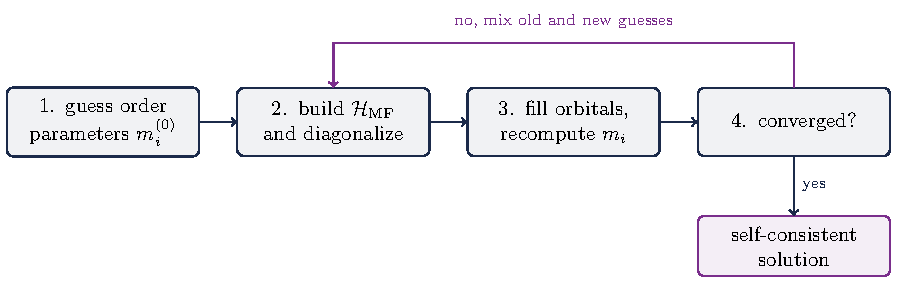
\includegraphics[width=0.95\textwidth]{figures/scf_loop.pdf}
  \caption{The self-consistency loop, which is what every mean-field calculation in this session
    actually runs. Steps 2 and 3 are the two halves that alternate: an order parameter fixes a
    single-particle Hamiltonian through Eq.~\eqref{eq:mfham}, and diagonalizing that Hamiltonian
    and filling its lowest orbitals up to the target electron number fixes a new order parameter.
    Convergence means the two agree to within a tolerance, and until they do we mix the old and
    new guesses and go around again.}
  \label{fig:scf-loop}
\end{figure}

\subsection{Mean-field theory as a variational method}
There is an equivalent, and arguably more illuminating, way to think about all of this. Suppose
we restrict the many-body ground state to be a single Slater determinant, $\ket{\Psi} =
\cre{a_1}\cre{a_2}\cdots\vac$, and we minimize $\expval{\Ham}$ over the choice of single-particle
orbitals $\{a_n\}$. Since $\HMF$ depends on $\expval{n_{i\sigma}}$, and $\expval{n_{i\sigma}}$
itself depends on the ground state of $\HMF$, minimizing the energy this way is precisely the
self-consistency loop we just described: guess $\{m_i\}$, diagonalize $\HMF$, recompute $\{m_i\}$
from the filled orbitals, and repeat until it converges. So mean-field theory is really the best
approximation we can build out of \emph{product states}, and that restriction to product states
is exactly what will get us into trouble in Section~\ref{sec:breakdown}.

\begin{notebook}
Section ``Magnetic order driven by interactions in a chain.'' Run the self-consistency loop for
a chain at fixed filling and look at the converged spin-up/spin-down bands: you should see one
cosine band per spin, split by the exchange field, with only the spin-down band occupied at the
filling used in the notebook.
\end{notebook}

\subsection{Gap opening at half filling}
Let us now force half filling and double the unit cell, so we have two sites with alternating
majority spin. At $U=0$ this just folds the metallic cosine band onto itself. Once $U>0$, the
self-consistent solution opens a gap between the occupied and empty bands, and that gap grows
with $U$, eventually becoming linear, $\Delta \sim U$, once $U \gg t$. If you look at the
single-particle spectral function instead of the eigenvalues, you see exactly the same story: a
continuous metallic density of states at $U=0$ develops a clean gap that widens with $U$, which
is precisely what a spectroscopy experiment would pick up.

\subsection{Multiple self-consistent solutions and their energetics}
Because the self-consistency loop is a \emph{nonlinear} fixed-point problem, the solution it
converges to depends on where we start it. A ferromagnetic initial guess converges to a
metallic, ferromagnetic solution; an antiferromagnetic initial guess converges to an insulating,
antiferromagnetic solution. Both of these are legitimate stationary points of the mean-field
energy, but only one of them is the true, lowest-energy mean-field ground state. If we take a
half-filled chain with only nearest-neighbor hopping, it turns out the antiferromagnetic
solution is always lower in energy, and the gap between the two scales as
\begin{equation}
  E_{\mathrm{FM}} - E_{\mathrm{AFM}} \;\sim\; \frac{1}{U} \xrightarrow{U\to\infty} 0.
\end{equation}
So the two solutions only become degenerate in the strict atomic limit $U\to\infty$; at any
finite $U$ they are physically distinct states, one metallic and one insulating.

\begin{notebook}
Section ``The interacting Hubbard dimer.'' Compare a ferromagnetic-seeded and an
antiferromagnetic-seeded self-consistent run on the dimer of Section~\ref{sec:dimer}, now with
$U>0$ switched on, and check numerically which solution has the lower variational energy and how
the gap between them scales with $U$. It is also worth revisiting ``Gap opening in the Hubbard
model'' with a ferromagnetic initialization, to see this initial-guess dependence show up
directly in the spectrum.
\end{notebook}

\section{The strong-coupling limit: from electrons to spins}
\label{sec:strongcoupling}
As $U/t \to \infty$, something nice happens to the local moment $\expval{n_{i\up}} -
\expval{n_{i\dn}}$: it saturates, in magnitude, to $1$ on every site. Double occupancy and empty
sites become energetically forbidden, and every site ends up carrying exactly one localized
electron. This is the regime where the physics is no longer best described by itinerant
fermions, but by \emph{spins}, and it is worth understanding in detail why.

\subsection{The Hubbard dimer and its low-energy manifold}
Take our two-site dimer again, with hopping $t$, interaction $U$, and two electrons total (so we
are at half filling). We already counted a six-dimensional many-body basis for this problem in
Section~\ref{sec:dimer}. For $U \gg t$, this basis splits cleanly into two groups:
\begin{itemize}[nosep]
  \item a four-dimensional \textbf{ground-state manifold} of singly-occupied configurations
    ($\up\dn$, $\dn\up$, $\up\up$, $\dn\dn$ across the two sites), sitting at energy $\sim 0$;
  \item a \textbf{virtual (high-energy) manifold} of doubly-occupied configurations, sitting at
    energy $\sim U$.
\end{itemize}
Look closely at the ground-state manifold: it is exactly the Hilbert space of two
spin-$\tfrac12$ degrees of freedom. In other words, our strongly interacting electronic problem
has quietly turned into a spin problem.

\subsection{Superexchange: $J = 4t^2/U$}
The only term that connects the two manifolds is the hopping $t$, and symmetry alone (there is
no spin-rotation breaking anywhere in $\Ham_{\mathrm{Hub}}$) already tells us that the low-energy
effective Hamiltonian has to be proportional to $\vb S_1\cdot\vb S_2$ at leading order in spin
operators. To actually pin down the coefficient, we treat $\Ham_0 = U\sum_i n_{i\up}n_{i\dn}$ as
the unperturbed Hamiltonian, with the singly- and doubly-occupied configurations of
Section~\ref{sec:dimer} as its eigenstates, and the hopping $V =
-t\sum_\sigma(\cre{0\sigma}\ann{1\sigma}+\mathrm{h.c.})$ as the perturbation. The parallel
configurations $\ket{\up\up}$ and $\ket{\dn\dn}$ have no doubly-occupied virtual state to hop into
at all, since Pauli exclusion blocks it, so they are exact eigenstates already, unshifted at any
order: this is our triplet, sitting at $E_{\mathrm{triplet}}=0$.

\begin{figure}[H]
  \centering
  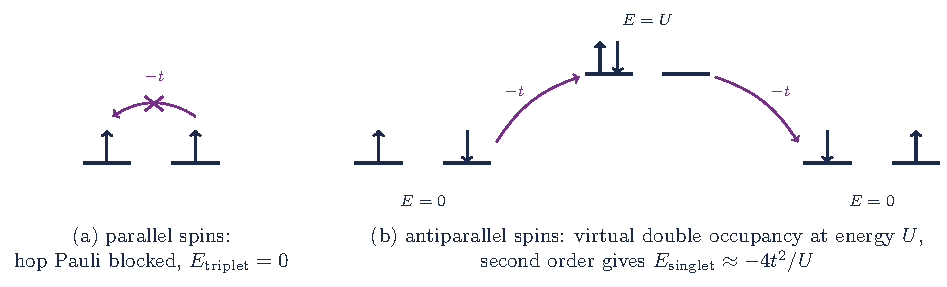
\includegraphics[width=0.92\textwidth]{figures/superexchange.pdf}
  \caption{The two spin channels of the half-filled Hubbard dimer at strong coupling, which is
    where the $J=4t^2/U$ of Eq.~\eqref{eq:superexchange} comes from. (a) With parallel spins there
    is no doubly-occupied state available to hop into, Pauli exclusion blocks the process outright,
    and the triplet stays exactly at $E_{\mathrm{triplet}}=0$ at every order. (b) With antiparallel
    spins either electron can hop onto its neighbor, passing through a virtual doubly-occupied
    configuration at energy $U$ and landing on the exchanged configuration. Each hop carries a
    matrix element $-t$ and the virtual state is paid for by an energy denominator $-U$, so
    second-order perturbation theory lowers the antiparallel channel by an amount of order
    $t^2/U$ while leaving the parallel one untouched.}
  \label{fig:superexchange}
\end{figure}

The antiparallel configurations are more subtle, since \emph{either} electron can hop, so each one
of $\ket{\up\dn} = \cre{0\up}\cre{1\dn}\vac$ and $\ket{\dn\up} = \cre{0\dn}\cre{1\up}\vac$ connects
through $V$ to \emph{both} virtual doubly-occupied states, $\ket{2,0} = \cre{0\up}\cre{0\dn}\vac$
and $\ket{0,2} = \cre{1\up}\cre{1\dn}\vac$, each sitting at energy $U$ above the low-energy
manifold, with matrix elements $\bra{2,0}V\ket{\up\dn} = -t$ and $\bra{0,2}V\ket{\up\dn}=-t$ (and,
by the site-exchange symmetry of the problem, $\bra{2,0}V\ket{\dn\up} = +t$,
$\bra{0,2}V\ket{\dn\up}=+t$, the sign flipping because of fermionic anticommutation once the two
electrons are reordered onto the same site). It is only the total spin, not the sublattice, that
is conserved here, so the clean way to organize the calculation is to work directly in the
singlet/triplet basis rather than $\{\ket{\up\dn},\ket{\dn\up}\}$. Only the singlet combination
$\ket{s}=\tfrac1{\sqrt2}(\ket{\up\dn}-\ket{\dn\up})$ has any overlap with the doubly-occupied
states at all (the triplet combination's matrix elements to $\ket{2,0}$ and $\ket{0,2}$ cancel by
the sign flip above), and by the same site-exchange symmetry only the symmetric combination
$\ket{d}=\tfrac1{\sqrt2}(\ket{2,0}+\ket{0,2})$ couples back to it, since the antisymmetric
combination $\tfrac1{\sqrt2}(\ket{2,0}-\ket{0,2})$ is odd under the mirror that $\ket s$ is even
under. Explicitly,
\begin{equation}
  \bra{d}V\ket{s} = \tfrac1{\sqrt2}\left[\bra{2,0}V\ket{\up\dn}-\bra{2,0}V\ket{\dn\up}
    +\bra{0,2}V\ket{\up\dn}-\bra{0,2}V\ket{\dn\up}\right]\tfrac1{\sqrt2}
  = \tfrac12\left[-t-t-t-t\right] = -2t,
\end{equation}
so the singlet sector reduces to an exact $2\times2$ problem, $\ket s$ at energy $0$ coupled to
$\ket d$ at energy $U$ by the matrix element $-2t$, with the orthogonal antisymmetric
doubly-occupied combination decoupled entirely, remaining an exact eigenstate at energy $U$.
Standard non-degenerate second-order (Schrieffer--Wolff, or equivalently L\"owdin) perturbation
theory on this $2\times2$ block gives
\begin{equation}
  E_{\mathrm{singlet}} \approx 0 + \frac{|\bra{d}V\ket s|^2}{0-U} = -\frac{4t^2}{U},
\end{equation}
which one can check is exactly the $U\gg t$ expansion of the closed-form eigenvalue of the full
$2\times2$ matrix, $E_-=\tfrac U2-\sqrt{(U/2)^2+4t^2}\to-4t^2/U$; a full numerical exact
diagonalization of the two-site, two-electron Hubbard model confirms both this asymptotic value
and the exact triplet energy $E_{\mathrm{triplet}}=0$ at every $U/t$, not just at strong coupling.
Compare this to the exact spectrum of $J\,\vb S_1\cdot\vb S_2$ itself: writing
$\vb S_{\mathrm{tot}}=\vb S_1+\vb S_2$ gives $\vb S_1\cdot\vb S_2 =
\tfrac12\left[S_{\mathrm{tot}}(S_{\mathrm{tot}}+1)-\tfrac34-\tfrac34\right]$, which evaluates to
$-\tfrac34$ for the singlet ($S_{\mathrm{tot}}=0$) and $+\tfrac14$ for the triplet
($S_{\mathrm{tot}}=1$), i.e.\ $E_{\mathrm{singlet}}=-\tfrac34J$ and $E_{\mathrm{triplet}}=\tfrac14J$,
a gap of exactly $J$ between them. Matching this gap to the one we just computed fixes
\begin{equation}
  J = E_{\mathrm{triplet}}-E_{\mathrm{singlet}} = \frac{4t^2}{U} \qquad\Longrightarrow\qquad
  \Ham_{\mathrm{eff}} = J\, \vb S_1\cdot\vb S_2,
  \label{eq:superexchange}
\end{equation}
the \textbf{antiferromagnetic superexchange} coupling. Intuitively: virtual hopping into the
doubly-occupied states, which is Pauli-blocked for parallel spins, lowers the energy of the
singlet combination of antiparallel configurations, and that is why the effective low-energy
interaction ends up favoring antialignment even though the underlying Hubbard repulsion has no
explicit spin dependence at all. The same argument goes through unchanged on an arbitrary lattice with hoppings
$t_{ij}$: the half-filled, strongly interacting Hubbard model on \emph{any} lattice maps onto a
spin-$\tfrac12$ \textbf{Heisenberg model},
\begin{equation}
  \Ham_{\mathrm{Heis}} = \sum_{ij} J_{ij}\, \vb S_i \cdot \vb S_j, \qquad J_{ij} \sim
  \frac{t_{ij}^2}{U}.
  \label{eq:heislattice}
\end{equation}
with the same numerical prefactor as Eq.~\eqref{eq:superexchange}, $J_{ij}=4t_{ij}^2/U$, for each
bond treated in isolation this way.
If instead we have more than one electron per site, as in multi-orbital atoms, we map onto
higher-spin Heisenberg models instead: spin-$1$ for two electrons per site, spin-$\tfrac32$ for
three, and so on. Additional weakly interacting orbitals can even flip the \emph{sign} of
$J_{ij}$, giving us ferromagnetic rather than antiferromagnetic coupling, which is worth keeping
in mind since real materials are not always antiferromagnets.

\begin{notebook}
Section ``The strongly interacting limit of the Hubbard model.'' Compute $E_{\mathrm{FM}} -
E_{\mathrm{AFM}}$ as a function of $U$ and check that it follows the $1/U$ scaling we derived
above. Then push to smaller $U$ and see where the perturbative assumption $t\ll U$ behind
Eq.~\eqref{eq:superexchange} starts to break down.
\end{notebook}

\section{Classical magnetic order and frustration}
If we now treat the spins in $\Ham_{\mathrm{Heis}}$ as classical vectors, an approximation that
is in spirit very close to mean-field theory itself, finding the ground state becomes a
straightforward energy minimization.

\paragraph{Bipartite lattices.} On the square and honeycomb lattices, we can always split the
sites into two sublattices $A, B$ such that every bond connects $A$ to $B$. For
antiferromagnetic $J>0$, the classical ground state is then simply $\vb S_A = -\vb S_B$:
collinear N\'eel order.

\paragraph{Frustration.} Things get more interesting on lattices that are \emph{not} bipartite,
like the triangular and kagome lattices, which are built out of corner- or edge-sharing
triangles. There, no assignment of two sublattices can satisfy every antiferromagnetic bond at
once. The classical ground state instead becomes \textbf{non-collinear}: neighboring spins
rotate by $120^\circ$ as you go around each triangle, producing a spiral magnetic order with a
multi-site magnetic unit cell.

\begin{figure}[H]
  \centering
  \begin{subfigure}[c]{0.32\textwidth}
    \centering
    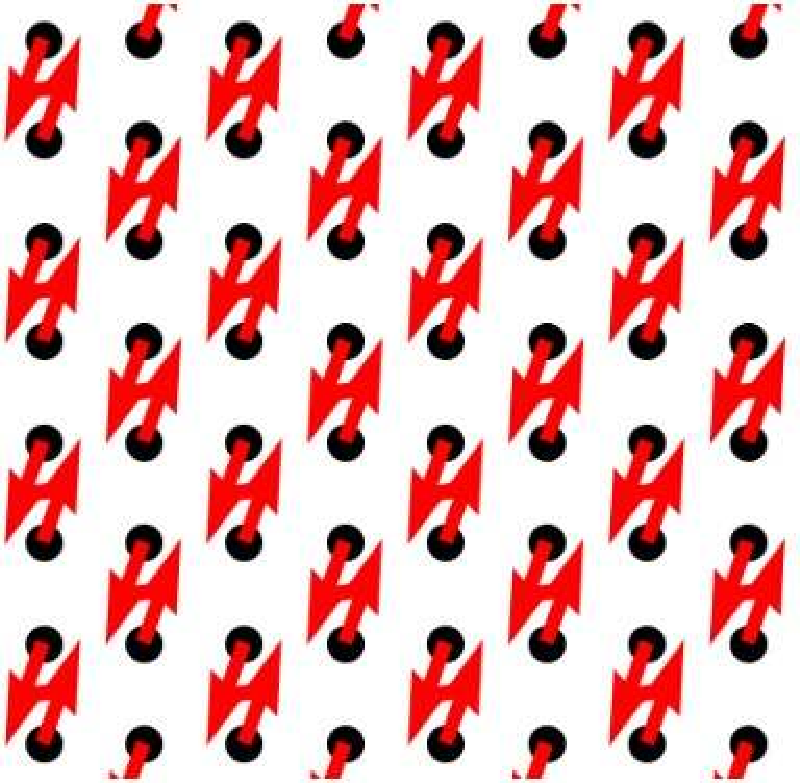
\includegraphics[width=\linewidth]{figures/classical_magnetism/neel_square_lattice.pdf}
    \caption{Bipartite square lattice}
  \end{subfigure}\hfill
  \begin{subfigure}[c]{0.53\textwidth}
    \centering
    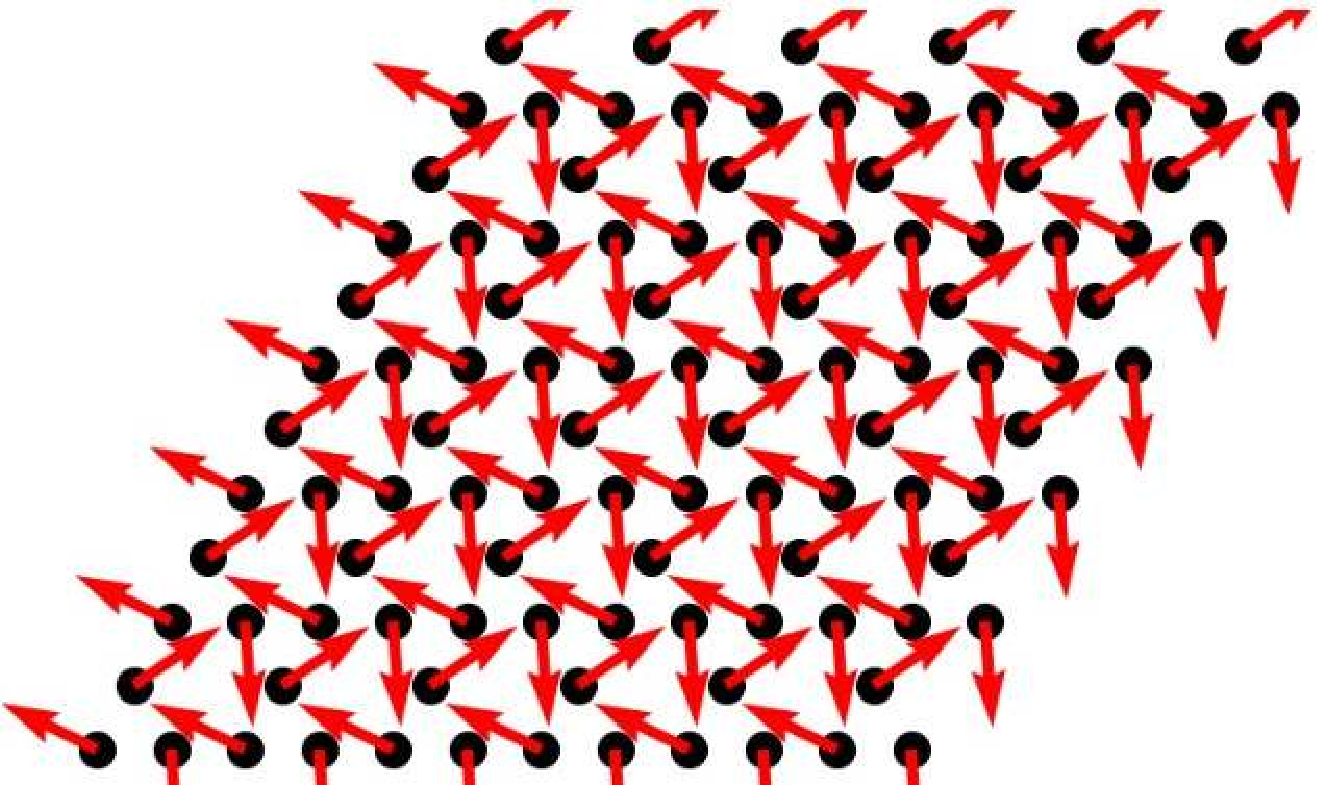
\includegraphics[width=\linewidth]{figures/classical_magnetism/spiral_triangular_lattice.pdf}
    \caption{Frustrated triangular lattice}
  \end{subfigure}
  \caption{Classical ground states of the Heisenberg model of Eq.~\eqref{eq:heislattice} with
    antiferromagnetic $J>0$, obtained by treating every spin as a classical vector. (a) On a
    bipartite lattice every bond connects the two sublattices, so $\vb S_A = -\vb S_B$ satisfies
    all of them simultaneously and the order is collinear N\'eel. (b) On the triangular lattice
    the bonds sit on corner-sharing triangles and no two-sublattice assignment can satisfy all of
    them, so the minimum-energy configuration is instead the non-collinear $120^\circ$ spiral,
    with a magnetic unit cell spanning several sites.}
  \label{fig:neel-vs-spiral}
\end{figure}

\begin{notebook}
Section ``Non-collinear magnetism in the Hubbard model from competing interactions'' and
``Non-collinear magnetic order from geometric frustration.'' Add a second-neighbor hopping to
the mean-field chain and see that it, too, can stabilize non-collinear order: competing exchange
paths play the same frustrating role as triangular geometry does. Then move to the
triangular/kagome supercells and read off the $120^\circ$ spiral directly from the
self-consistent magnetization pattern.
\end{notebook}

\paragraph{Anisotropic exchange.} Real materials often break the SU(2) spin-rotation symmetry of
$\Ham_{\mathrm{Heis}}$ through spin--orbit coupling, adding bilinear-in-spin terms that are
\emph{not} symmetric under a common rotation of all spins. There are three that come up often
enough to be worth naming:
\begin{itemize}[nosep]
  \item \textbf{Antisymmetric (Dzyaloshinskii--Moriya) exchange}, $\vb D_{ij}\cdot(\vb S_i\times
    \vb S_j)$, which shows up when mirror symmetry is broken and favors spins sitting at
    $90^\circ$ to each other, i.e.\ non-collinear order even without any geometric frustration.
  \item \textbf{Ising anisotropy}, coupling only $S_i^z S_j^z$, which arises from strong
    spin--orbit coupling and single-ion anisotropy and pushes the spins toward classical
    behavior, confined to a single axis or plane.
  \item \textbf{Kitaev exchange}, a \emph{bond-dependent} Ising-like coupling where $x$-bonds
    couple $S^xS^x$, $y$-bonds couple $S^yS^y$, and $z$-bonds couple $S^zS^z$. No single spin
    configuration can satisfy all three bond types at once on, say, the honeycomb lattice, which
    is exactly why this term is intrinsically frustrating and a key ingredient behind quantum
    spin liquid models.
\end{itemize}
None of these three terms are covered in the companion notebook. We flag them here as
slides-only material that becomes relevant again in more advanced treatments of quantum
magnetism.

\section{Charge density waves as a mean-field problem}
The very same machinery applies to $\Ham_{\mathrm{CDW}}$ from Eq.~\eqref{eq:cdwmodel}: we
decouple the density--density term via $\expval{n_i} n_{i+1} + n_i\expval{n_{i+1}} -
\expval{n_i}\expval{n_{i+1}}$ and iterate to self-consistency, exactly as before. At $V=0$ the
chain is a featureless, half-filled metal with $n_i = \tfrac12$ on every site. As we turn on $V$,
we get exactly the same qualitative spectral evolution as in the Hubbard case: a gap opens and
grows $\sim V$ at large $V$. What changes is the order parameter, which is now the
\textbf{charge imbalance},
\begin{equation}
  \delta n \equiv n_{\text{even}} - n_{\text{odd}},
\end{equation}
and it grows from $0$ at $V=0$ toward $\delta n \to 1$ at large $V$, meaning the sites end up
alternating fully filled and fully empty. The broken symmetry here is translational rather than
time-reversal, but notice how closely the mechanism, and even the shape of the spectral
evolution, mirrors the magnetic case.

\begin{notebook}
Sections ``Gap opening in a spinless interacting model'' and ``Symmetry breaking in the spinless
fermionic chain.'' Track the gap and the charge imbalance $\delta n$ as a function of $V$, then
seed the self-consistency loop with an explicit external CDW field and see how it selects which
sublattice orders.
\end{notebook}

\section{Where mean-field theory breaks down}
\label{sec:breakdown}
So far mean-field theory has worked well every time, and that is really because it is a very
good technique precisely when the true ground state \emph{does} spontaneously break a symmetry.
But nothing guarantees this in advance, and the Hubbard dimer at half filling gives us a clean
counterexample.

The exact Hamiltonian $\Ham_{\mathrm{Hub}}$ for two sites is fully spin-rotation and
time-reversal symmetric. Its mean-field decoupling, however, is only self-consistent with a
\emph{symmetry-breaking} ansatz once $U$ passes a threshold: below threshold, $\HMF$ stays
non-magnetic, and above it, the converged solution has finite, eventually saturating local
moments of opposite sign on the two sites, exactly the regime we studied in
Section~\ref{sec:strongcoupling}. The mean-field gap tracks this transition too, staying
constant below threshold and then growing linearly above it.

Now compare this to the \emph{exact} many-body ground state, and the story looks quite
different. In the strongly interacting limit, Section~\ref{sec:strongcoupling} already told us
the dimer maps onto $\Ham_{\mathrm{eff}} = J\,\vb S_1\cdot\vb S_2$, and we can just diagonalize
that by hand: its exact ground state is the singlet
\begin{equation}
  \ket{\Psi_{\mathrm{singlet}}} = \frac{1}{\sqrt2}\Big(\ket{\up\dn} - \ket{\dn\up}\Big).
\end{equation}
This state has $\expval{S_1^z} = \expval{S_2^z} = 0$. It simply does not break time-reversal
symmetry, in direct conflict with what the symmetry-broken mean-field solution told us to
expect. The reason is structural, not a numerical accident: $\ket{\Psi_{\mathrm{singlet}}}$ is
an entangled superposition, and it cannot be written as any single Slater determinant, no matter
what choice of orbitals or spin quantization axis we try. Mean-field theory, built by
construction out of product states (Section~\ref{sec:strongcoupling}), can simply never reach
it.

\paragraph{Why this matters.} The Hubbard dimer is the smallest Hamiltonian you can write down
that shows this failure mode, but the failure itself is completely generic: whenever the true
many-body ground state is genuinely entangled and not adiabatically connected to a product
state, mean-field theory gets the physics qualitatively wrong, the wrong symmetry, the wrong
order, sometimes an entirely wrong phase. This is exactly the agenda for the rest of the course:
\emph{exact diagonalization} (Sessions 2--3) solves small many-body Hamiltonians with no
product-state restriction at all, and \emph{tensor network} methods (Sessions 4--5) let us
recover the exact answer at system sizes where exact diagonalization is no longer feasible.

\begin{table}[H]
\centering
\small
\begin{tabular}{@{}P{3.1cm}P{3.9cm}P{3.9cm}P{3.9cm}@{}}
\toprule
 & \textbf{Mean-field theory} & \textbf{Exact diagonalization} & \textbf{Tensor networks (MPS)} \\
\midrule
Ansatz & product state (Slater det.) & unrestricted, full Hilbert space & bounded-entanglement
state (MPS) \\
Cost vs.\ size $L$ & polynomial & exponential, $\sim 2^L$ & polynomial in $L$ and bond dimension \\
Captures entanglement? & no & yes, exactly & yes, up to the bond dimension \\
Typical reach & any $L$ & $L \lesssim 20$--$30$ & $L \sim 40$--$100+$ (1D) \\
Fails when\ldots & ground state is not adiabatically connected to a product state (this session) &
never, in principle (only limited by $L$) & entanglement exceeds what the bond dimension can
store \\
\bottomrule
\end{tabular}
\caption{The three methods used in this course, previewed side by side: their ansatz, cost
scaling with system size $L$, whether they capture entanglement, typical reach, and failure
mode.}
\label{tab:methodpreview}
\end{table}

Think of Table~\ref{tab:methodpreview} as a preview rather than a derivation: we will develop and
use each of these methods on its own terms starting next session.

\section*{Summary}
\begin{itemize}[nosep]
  \item Second quantization lets us write single-particle and many-body ($\Order{4}$-fermion)
    Hamiltonians in one language; the interaction term is what drives all correlated physics.
  \item Mean-field theory decouples the interaction into an effective single-particle problem
    that we solve self-consistently; equivalently, it is a variational search over Slater
    determinants.
  \item The Hubbard model gives us magnetism (broken time-reversal/spin symmetry); the spinless
    nearest-neighbor model gives us charge density waves (broken translational symmetry), and
    both come from essentially the same mean-field mechanism.
  \item In the strongly interacting limit, second-order perturbation theory maps the Hubbard
    model onto a Heisenberg spin model with $J\sim t^2/U$, the superexchange coupling.
    Classically this model shows collinear order on bipartite lattices and
    non-collinear/frustrated order otherwise.
  \item Mean-field theory can fail qualitatively whenever the true ground state is entangled
    beyond any product state, exactly as we saw for the Hubbard dimer's singlet ground state.
    That failure is what motivates exact diagonalization and tensor networks, which we take up
    next session.
\end{itemize}

\end{document}
